\documentclass[10pt,twocolumn]{article}
\usepackage{geometry}
\geometry{verbose,headsep=3cm,tmargin=2.5cm,bmargin=2.5cm,lmargin=2.0cm,rmargin=2.0cm}
\usepackage{graphicx}
\usepackage{xcolor}
\usepackage[font=small]{caption}
\usepackage{amsmath,amssymb,latexsym}
\usepackage{marvosym}
\usepackage{url}
\usepackage{lipsum}
\usepackage{bm}
\usepackage{float}
\usepackage[english]{babel}
\usepackage{hyperref}
\usepackage{subcaption}
\usepackage{subfloat}
\usepackage{epsf}
\usepackage{float}
\usepackage{mathpazo}
\usepackage{pifont}
\usepackage{wrapfig}
\usepackage{multicol}
\usepackage{enumitem}
\usepackage{xcolor}
\usepackage{framed}
\usepackage[utf8]{inputenc}
\graphicspath{{DWGs/}}
\usepackage{framed}
\usepackage{textcomp}
\usepackage{braket}
\newcommand{\highlight}[1]{%
  \colorbox{orange!50}{$\displaystyle#1$}}
% Default fixed font does not support bold face
\DeclareFixedFont{\ttb}{T1}{txtt}{bx}{n}{10} % for bold
\DeclareFixedFont{\ttm}{T1}{txtt}{m}{n}{10}  % for normal

% Custom colors
\usepackage{color}
\definecolor{deepblue}{rgb}{0,0,0.5}
\definecolor{deepred}{rgb}{0.6,0,0}
\definecolor{deepgreen}{rgb}{0,0.5,0}

\usepackage{listings}

% Python style for highlighting
\newcommand\pythonstyle{\lstset{
language=Python,
basicstyle=\ttm,
otherkeywords={self},             % Add keywords here
keywordstyle=\ttb\color{deepblue},
emph={MyClass,__init__},          % Custom highlighting
emphstyle=\ttb\color{deepred},    % Custom highlighting style
stringstyle=\color{deepgreen},
frame=tb,                         % Any extra options here
showstringspaces=false            % 
}}


% Python environment
\lstnewenvironment{python}[1][]
{
\pythonstyle
\lstset{#1}
}
{}

% Python for external files
\newcommand\pythonexternal[2][]{{
\pythonstyle
\lstinputlisting[#1]{#2}}}

% Python for inline
\newcommand\pythoninline[1]{{\pythonstyle\lstinline!#1!}}
% Document font:
\usepackage{charter}

\begin{document}

%%% HEADER --------------------------------------------------------------
% ------------------------------------------------------------------------

\twocolumn[{
\begin{@twocolumnfalse}

  \begin{center}
%\textcolor{lgray}
    \vskip-5em

    \hfill
    \fontsize{10}{10}\selectfont {\textit{Bruxelles, April 2019}}
    \vskip2ex
	\vspace{5ex}
    \fontsize{20}{10}\selectfont {Quality of reconstruction measures}
      \vspace{1ex}
      
  \noindent%
    
\vskip1ex

{\rule{\textwidth}{0.5pt}}

  \end{center}
  
    \fontsize{7}{10}\selectfont {This work is licensed under the Creative Commons Attribution-NonCommercial-ShareAlike 4.0 International (CC BY-NC-SA 4.0) license.}

\vspace{6mm}

\end{@twocolumnfalse}
}]

%%% HEADER END -----------------------------------------------------------
% ------------------------------------------------------------------------

\vspace{10mm}

\setlength{\parindent}{0cm}

\fontsize{14}{10}\selectfont {Kamila Zdybał}

\vspace{2mm}

\fontsize{8}{10}\selectfont {\textit{Université libre de Bruxelles, kamila.zdybal@ulb.ac.be}}

\fontsize{8}{10}\selectfont {\textit{camillejr.github.io/science-docs, kamila.zdybal@gmail.com}}

\section*{Preface}

These are notes on measures of the quality of reconstruction.

This document is still in preparation. Please feel free to contact me with any suggestions, corrections or comments.

\section*{Keywords}

\textit{principal component analysis, data reduction, dimensionality reduction, linear algebra, MATLAB\textregistered, Python}

\tableofcontents

\section{Nomenclature}

\begin{tabular}{ll}
    $\bm{A}$ & is a matrix \\
     $\bm{A}^T$ & denotes a matrix transpose \\
    $A_{:,j}$ & is a vector formed by the $j^{th}$ column of a matrix $\bm{A}$, \\
    & it is equivalent to  $\bm{A}(:,j)$ \\
    $A_{i,:}$ & is a vector formed by the $i^{th}$ row of a matrix $\bm{A}$, \\
    & it is equivalent to  $\bm{A}(i,:)$ \\
    $a_{i,j}$ & is an element from $i^{th}$ row and $j^{th}$ column of a matrix $\bm{A}$, \\ 
    & it is equivalent to  $\bm{A}(i,j)$ \\
\end{tabular}


\section{Coefficient of determination}

\section{Root mean squared error (RMSE)}


\begin{equation}
RMSE_i = \sqrt{\overline{(\bm{X}_i - \bm{f}_i)^2}}
\end{equation}

\subsection{Normalized root mean squared error (NRMSE)}

\begin{equation}
NRMSE_i = \sqrt{\frac{\overline{(\bm{X}_i - \bm{f}_i)^2}}{\overline{\bm{X}_i^2}}}
\end{equation}


\begin{figure}[H]
\centering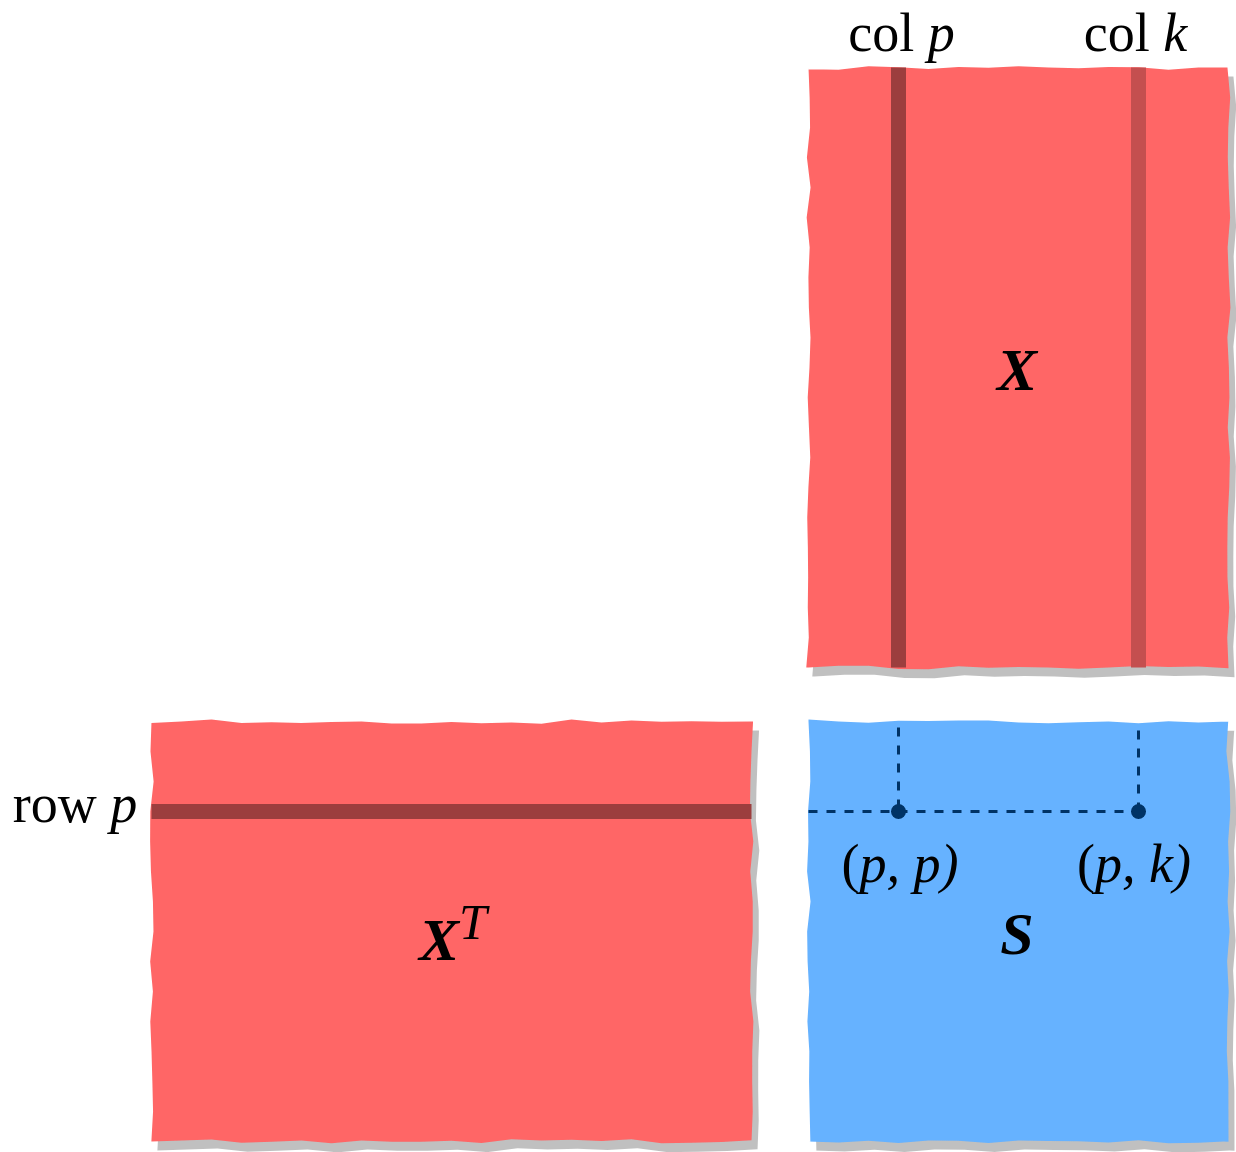
\includegraphics[width=7cm]{cov-matrix.png}
\caption{Covariance matrix $\bm{S}$ graphical interpretation.}
\label{fig:covariance-matrix}
\end{figure}


\begin{python}
q = 1
Dataset_projected = np.dot(Dataset_proc,
np.transpose(pca.components_[:q,:]))
\end{python}


\appendix



\section{Appendix}
\thebibliography{}


\end{document}
